\chapter{Space System}

\section{Overview}

The highest level system of a space mission is termed the space system. Examples are: the Global Positioning System (GPS), the European Data Relay System (EDRS), or Disaster Monitoring Constellation for International Imaging (DMCii), to name a few.

The further breakdown of a typical space system is provided provided in ECSS-S-ST-00-01 \cite{ECSS-S-ST-00-01} as follows. First, the space system is functionally categorized into three segments: space segment, ground segment, and launch segment. Each segment is further decomposed as shown exemplary for the space segment:

\begin{itemize}
\item space segment (functional)
\item space segment system (functional)
\item space segment element 
\item space segment subsystem (functional)
\item space segment equipment/unit
\item components/parts
\end{itemize}

Functional elements are logical grouping of physical elements. Figure \ref{fig:Space System Breakdown Schema} visualizes the ECSS approach for achieving a breakdown of the system.

\begin{figure}[h]
\centering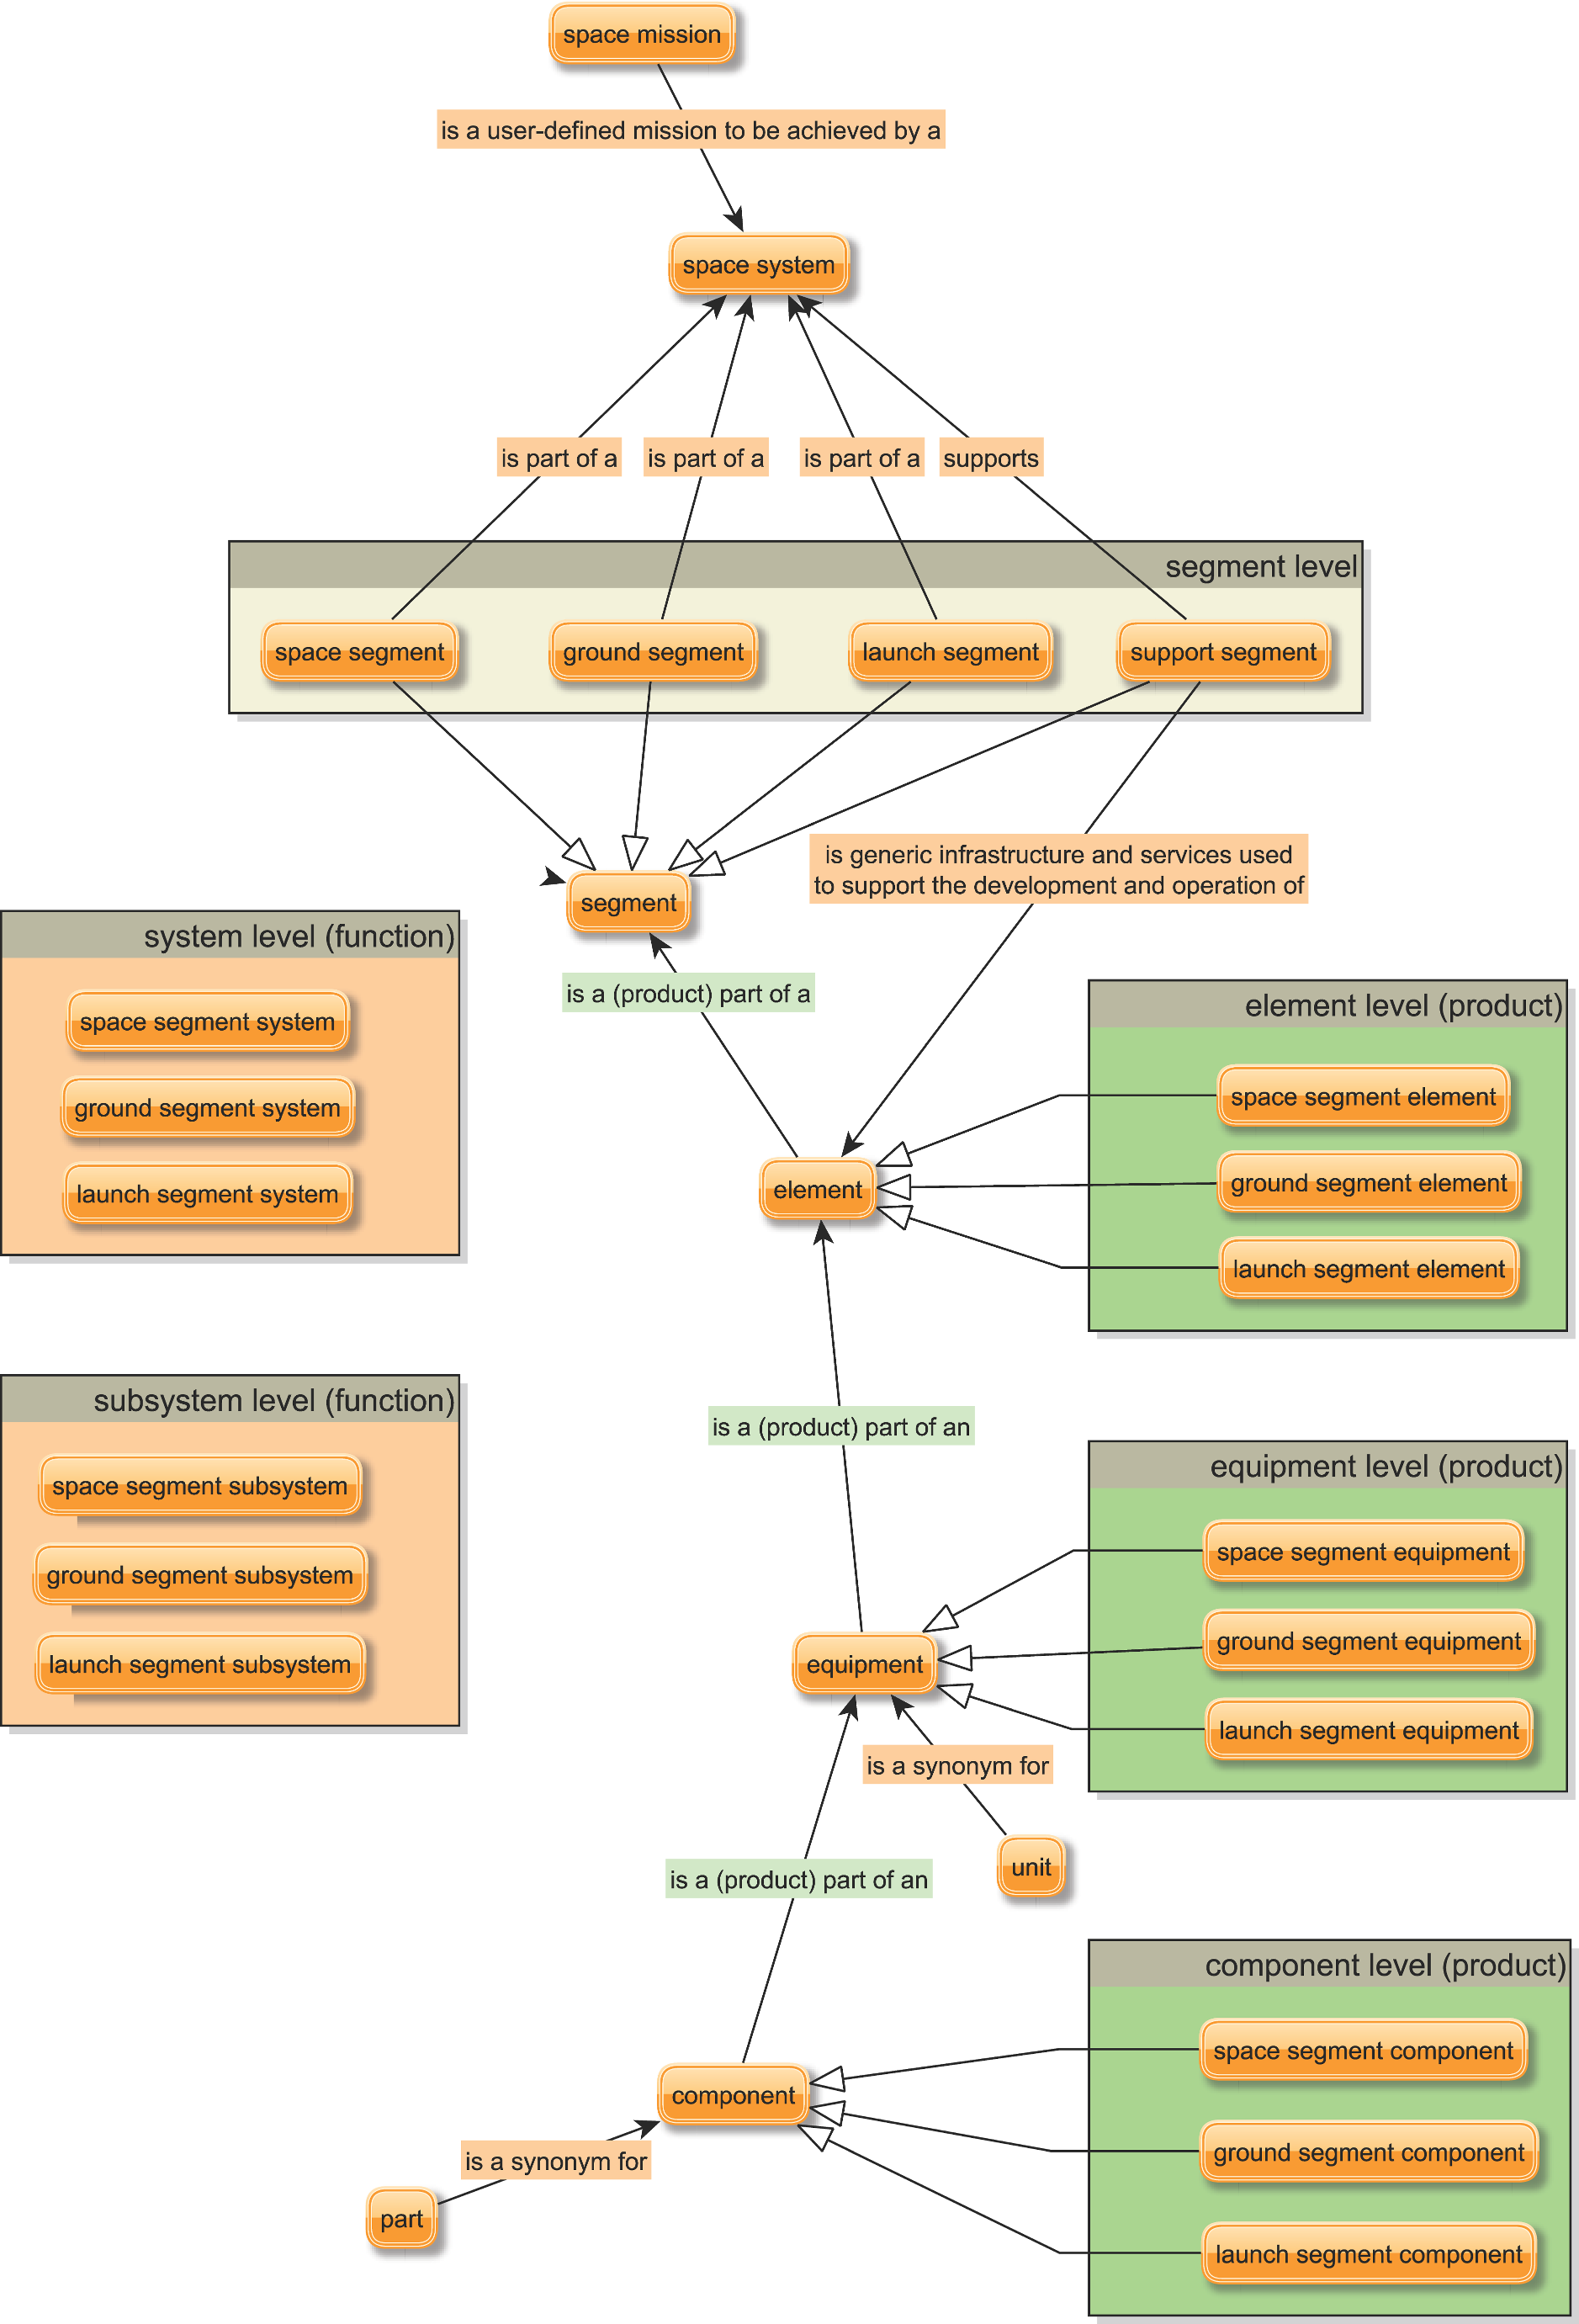
\includegraphics[width=1.0\linewidth]{fig/system_decomposition}
\caption{Space System Breakdown Schema (copyright ECSS)}
\label{fig:Space System Breakdown Schema}
\end{figure}

\section{Formats}

There are almost no standards that are applicable to the entire space system as such. Of those that are, the are concerned with formats of data to be used across the segment boundaries.

\subsection{Time}

\begin{tabular}{l}
\textit{CCSDS 301.0-B "Time Code Formats" \cite{CCSDS-301.0-B}} \\
\end{tabular}

Time codes are digital representations of time information. Four time codes are available: one unsegmented and three segmented time codes. All use the international standard second as the fundamental unit of time. An unsegmented time code is a pure binary count of time units and fractional time units from a starting time called the epoch. A segmented time code is one in which the count of time units and fractional time units is accumulated in two or more cascaded counters which count modulo of various bases and start from the epoch. 

The \textbf{CCSDS unsegmented time code} (CUC) consists of a number of contiguous octets representing an integrated  number of the basic time unit from a defined epoch along with an optional integer number of octets representing the elapsed binary fraction of the basic time unit. The time code increases monotonically without reversion. The CCSDS-Recommended epoch is that of 1958 January 1 and the recommended time unit is the second, using TAI as reference time scale. This time code is not UTC-based and leap-second corrections do not apply. 

The \textbf{CCSDS day segmented time code} (CDS) consists of a 16 or 24 bit counter for the day from epoch, a 32 bit counter for the milliseconds of the day and optionally a 16/32 bit counter for the submilliseconds. The CCSDS recommended day segment is a continuous counter of days from 1958 January 1 starting with 0. Since this code is UTC-based, the leap second correction must be made. 

The \textbf{CCSDS calendar segmented time code} (CCS) is defined in month of year / day of month format, or as day of year format. Both CCS time code variations are UTC-based. The leap second correction must be made.

The \textbf{CCSDS ASCII segmented  time code} is composed of a variable number of ASCII 
characters and defined in month of year / day of month format, or as day of year format. Both ASCII time code variations are UTC-based and leap second corrections must be made. The time represented is intended to match civil time usage.  Therefore, the epoch is taken to be the usual Gregorian calendar epoch of 1 AD, and the time is that of the prime meridian. The format is:

ASCII time code A: YYYY-MM-DDThh:mm:ss.d$\rightarrow$dZ (e.g. 1988-01-18T17:20:43.123456Z)
ASCII time code B: YYYY-DDDThh:mm:ss.d$\rightarrow$dZ (e.g. 1988-018T17:20:43.123456Z)

where:

\begin{tabular}{l l}
DDD & is day of year, \\
T & is the calendar-time separator, \\
d$\rightarrow$d & is decimal fraction of second, and \\
Z & is the optional time code terminator.
\end{tabular}
 
\subsection{Identifiers}

\begin{tabular}{l}
\textit{CCSDS 320.0-B "CCSDS Global Spacecraft Identification Field..." \cite{CCSDS-320.0-B}} \\
\end{tabular}

The CCSDS SCID (spacecraft identifier) is a 10-bit number used in telecommand and telemetry frames and serves as a mechanism for the identification of a simple spacecraft having only one logical space-ground link; or an association between space-based and ground-based application processes with complex spacecraft having more than one logical space-ground link.

CCSDS has established the Space Assigned Numbers Authority (SANA) \cite{sanaregistry.org}, which coordinates the issuing of SCID to different spacecraft. It has the objective to eliminate the possibility that data from any given CCSDS-compatible vehicle will be falsely interpreted as being from another CCSDS-compatible vehicle or commands sent to a CCSDS-compatible vehicle will be received and acted upon by application processes for which they were not intended.
